\section{\bench{}}

We introduce \bench{}, a diagnostic evaluation suite for post-admission memory validity revision. Unlike existing evaluations that assess memory quality through downstream task success, \bench{} directly audits the record-level validity state of the agent's memory store.

\paragraph{Dataset Composition and Statistics.}
The dataset contains a total of $4,000$ scenarios:
\begin{itemize}[leftmargin=*]
\item \textbf{L3 Development Split ($3,500$ cases):} Designed for prompt engineering, schema validation, Guard testing, ablation development, controlled corruption generation, and future supervised training.
\item \textbf{L4 Held-Out Split ($500$ cases):} Disjoint in templates and domains from L3, serving as the sole official evaluation split.
\end{itemize}
The scenarios span six diverse domains (software engineering, task management, data analysis, enterprise tooling, customer support, and scientific work) and are structured using stable, semantic-free identifiers.

\begin{figure*}[t]
\centering
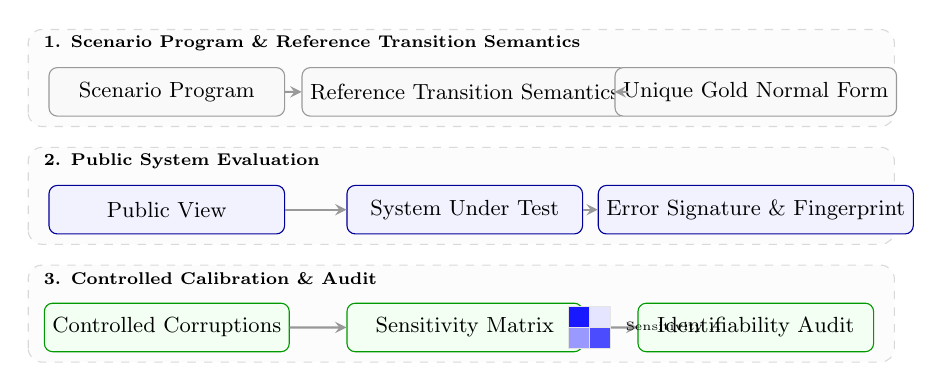
\begin{tikzpicture}[
    scale=0.88, every node/.style={transform shape},
    box/.style={rectangle, draw=gray!80, fill=gray!5, rounded corners=3pt, minimum width=3.4cm, minimum height=0.7cm, align=center, font=\small},
    bluebox/.style={rectangle, draw=blue!60!black, fill=blue!5, rounded corners=3pt, minimum width=3.4cm, minimum height=0.7cm, align=center, font=\small},
    greenbox/.style={rectangle, draw=green!60!black, fill=green!5, rounded corners=3pt, minimum width=3.4cm, minimum height=0.7cm, align=center, font=\small},
    arrow/.style={->, >=stealth, thick, draw=gray!80}
]

% Part 1: Gold Semantics
\draw[gray!30, fill=gray!2, dashed, rounded corners=5pt] (-0.5,1.2) rectangle (12.0,2.6);
\node[anchor=west, font=\bfseries\scriptsize] at (-0.4,2.4) {1. Scenario Program \& Reference Transition Semantics};
\node[box] (g1) at (1.5,1.7) {Scenario Program};
\node[box] (g2) at (5.8,1.7) {Reference Transition Semantics};
\node[box] (g3) at (10.0,1.7) {Unique Gold Normal Form};
\draw[arrow] (g1) -- (g2);
\draw[arrow] (g2) -- (g3);

% Part 2: System Evaluation
\draw[gray!30, fill=gray!2, dashed, rounded corners=5pt] (-0.5,-0.5) rectangle (12.0,0.9);
\node[anchor=west, font=\bfseries\scriptsize] at (-0.4,0.7) {2. Public System Evaluation};
\node[bluebox] (s1) at (1.5,0) {Public View};
\node[bluebox] (s2) at (5.8,0) {System Under Test};
\node[bluebox] (s3) at (10.0,0) {Error Signature \& Fingerprint};
\draw[arrow] (s1) -- (s2);
\draw[arrow] (s2) -- (s3);

% Part 3: Calibration & Audit
\draw[gray!30, fill=gray!2, dashed, rounded corners=5pt] (-0.5,-2.2) rectangle (12.0,-0.8);
\node[anchor=west, font=\bfseries\scriptsize] at (-0.4,-1.0) {3. Controlled Calibration \& Audit};
\node[greenbox] (c1) at (1.5,-1.7) {Controlled Corruptions};
\node[greenbox] (c2) at (5.8,-1.7) {Sensitivity Matrix};
\node[greenbox] (c3) at (10.0,-1.7) {Identifiability Audit};
\draw[arrow] (c1) -- (c2);
\draw[arrow] (c2) -- (c3);

% Small Heatmap inset in Part 3
\begin{scope}[shift={(7.3,-2.0)}]
    \draw[fill=blue!90, draw=gray!20] (0,0.3) rectangle (0.3,0.6);
    \draw[fill=blue!10, draw=gray!20] (0.3,0.3) rectangle (0.6,0.6);
    \draw[fill=blue!40, draw=gray!20] (0,0) rectangle (0.3,0.3);
    \draw[fill=blue!70, draw=gray!20] (0.3,0) rectangle (0.6,0.3);
    \node[right, font=\tiny] at (0.7,0.3) {Sensitivity $A$};
\end{scope}

\end{tikzpicture}
\caption{MemPatch-Bench evaluation protocol and diagnostic calibration pipeline. Raw programs yield a unique gold normal form under reference semantics. Agent outputs on public views produce multi-dimensional error signatures audited via controlled calibration.}
\label{fig:benchmark_pipeline}
\end{figure*}

\paragraph{Seven Memory Integration Failure Modes.}
Each scenario in \bench{} targets one of seven structural memory integration failures:
\begin{enumerate}[leftmargin=*]
\item \textbf{Stale-Reuse:} Obsolete records remain licensed for downstream reuse after contradictory evidence arrives.
\item \textbf{Under-Update:} Failure to identify and modify records targeted by valid updates.
\item \textbf{Conflict Collapse:} Concurrent contradictory updates leave the memory in an inconsistent, unresolved state without proper fail-closed logging.
\item \textbf{Scope Leakage:} Contextual or domain-specific exclusions are ignored, leaking out-of-scope records into active reasoning.
\item \textbf{Wrong-Source Attribution:} Crediting updates to incorrect or ungrounded evidence events.
\item \textbf{Policy Violation:} Violating safety, retention, or privacy constraints during memory modification.
\item \textbf{Memory Hallucination:} Proposing modifications to records that do not exist or using non-existent evidence identifiers.
\end{enumerate}

\paragraph{Evaluation Protocol.}
The evaluation protocol strictly isolates the hidden gold labels from the agent. The evaluator is fully deterministic, scoring output tuples $r = (d, \mathbf{s}, Z, f, a)$ to populate the diagnostic response matrix. Under Theorem~\ref{thm:gold_determinacy}, every valid scenario has a unique normal form determined by the transition rules, preventing shortcuts from masking state defects.

To enforce statistical rigor, \bench{} aggregates scenarios into hierarchical clusters defined by their underlying \emph{template family}. The L4 evaluation split comprises 500 instances partitioned into 18 unique template families, stratified across the seven failure modes: wrong source attribution (2 families, 75 instances), scope leakage (2 families, 75 instances), under-update (2 families, 87 instances), conflict collapse (6 families, 124 instances), policy violation (2 families, 63 instances), stale memory reuse (2 families, 42 instances), and memory hallucination (2 families, 34 instances). To account for intra-family correlations and establish robust statistical significance, we construct simultaneous confidence bounds for agent error rates using a paired cluster bootstrap. In each bootstrap replication, we resample entire template families (clusters) with replacement, preserving the joint distribution of instances within each cluster to compute distribution-free confidence intervals.

\paragraph{Metamorphic Equivariance Verification.}
To ensure the robustness of evaluations against spurious contextual or naming variations, we implement metamorphic testing to audit system equivariance under three transformations: (1) \emph{Record-ID Bijection (ID Renaming)}: mapping all memory and event identifiers via a random bijection, verifying that the output mapping scales equivariantly; (2) \emph{Irrelevant Event Insertion}: inserting non-causal heartbeat comments randomly into the trace; and (3) \emph{Distractor Reordering}: shuffling background distractors. The benchmark requires that any valid mediator maintains strict equivariance (zero equivariance defect) under these transformations, preventing models from relying on hardcoded identifier names or position biases.

